\documentclass[12pt,a4paper]{article}

\usepackage[utf8]{inputenc}
\usepackage[T1]{fontenc}
\usepackage[margin=2.3cm]{geometry}
\usepackage{amsmath,amssymb}
\usepackage{xcolor}
\usepackage{tikz}
\usepackage{graphicx}
\usepackage{listings}

\usetikzlibrary{arrows.meta,positioning,calc,fit}

\definecolor{loadcolor}{HTML}{FF5722}
\definecolor{soilcolor}{HTML}{8D6E63}
\definecolor{pilecolor}{HTML}{2196F3}
\definecolor{fusioncolor}{HTML}{9C27B0}

\lstset{
  basicstyle=\ttfamily\small,
  keywordstyle=\color{blue!80!black}\bfseries,
  commentstyle=\color{green!45!black}\itshape,
  stringstyle=\color{red!70!black},
  backgroundcolor=\color{gray!8},
  frame=single,
  framerule=0.4pt,
  breaklines=true,
  language=Python
}

\title{\textbf{Thermodynamic 21-Slot Model}\\[0.2em]
\large Code Explanation + Concept (Graphical)}
\author{PFE Research Notes}
\date{March 2026}

\begin{document}
\maketitle

% ===========================================================
\section{Core Concept (Graphical View)}
% ===========================================================

\begin{figure}[htbp]
\centering
\resizebox{0.98\textwidth}{!}{%
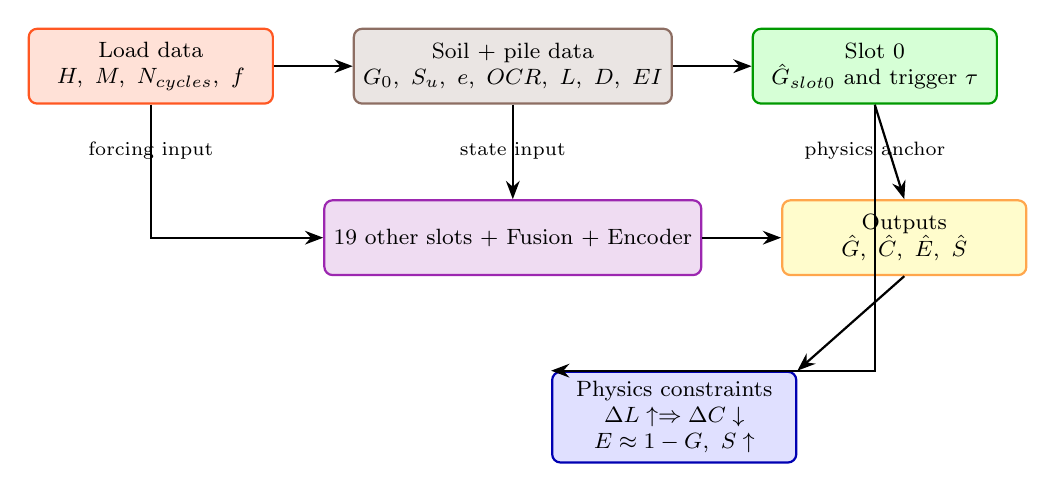
\begin{tikzpicture}[
  node distance=1.1cm and 1.0cm,
  box/.style={rectangle,rounded corners=3pt,draw,thick,minimum height=0.95cm,minimum width=3.1cm,align=center,font=\footnotesize},
  arr/.style={->,thick,>=Stealth},
  note/.style={font=\scriptsize,align=center}
]
\node[box,fill=loadcolor!18,draw=loadcolor] (load) {Load data\\$H,\ M,\ N_{cycles},\ f$};
\node[box,fill=soilcolor!18,draw=soilcolor,right=1.0cm of load] (soil) {Soil + pile data\\$G_0,\ S_u,\ e,\ OCR,\ L,\ D,\ EI$};
\node[box,fill=green!16,draw=green!60!black,right=1.0cm of soil] (slot0) {Slot 0\\$\hat{G}_{slot0}$ and trigger $\tau$};

\node[box,fill=fusioncolor!16,draw=fusioncolor,below=1.2cm of soil] (fusion) {19 other slots + Fusion + Encoder};
\node[box,fill=yellow!20,draw=orange!70,right=1.0cm of fusion] (heads) {Outputs\\$\hat{G},\ \hat{C},\ \hat{E},\ \hat{S}$};
\node[box,fill=blue!12,draw=blue!70!black,below=1.2cm of fusion,xshift=2.05cm] (physics) {Physics constraints\\$\Delta L\uparrow \Rightarrow \Delta C\downarrow$\\$E\approx1-G,\ S\uparrow$};

\draw[arr] (load) -- (soil);
\draw[arr] (soil) -- (slot0);
\draw[arr] (load.south) |- (fusion.west);
\draw[arr] (soil.south) -- (fusion.north);
\draw[arr] (slot0.south) -- (heads.north);
\draw[arr] (fusion) -- (heads);
\draw[arr] (heads.south) -- (physics.north east);
\draw[arr] (slot0.south) |- (physics.north west);

\node[note,below=0.35cm of load] {forcing input};
\node[note,below=0.35cm of soil] {state input};
\node[note,below=0.35cm of slot0] {physics anchor};
\end{tikzpicture}%
}
\caption{Main concept: Slot 0 gives physics-guided prediction and trigger, fusion gives global context, and losses enforce thermodynamics.}
\end{figure}

\textbf{In one sentence:} the model predicts $G/G_{\max}$ mainly from a dedicated physics slot (Slot 0), then refines with multi-slot fusion while enforcing physically consistent behavior.

% ===========================================================
\section{Code Structure Map (Graphical)}
% ===========================================================

\begin{figure}[htbp]
\centering
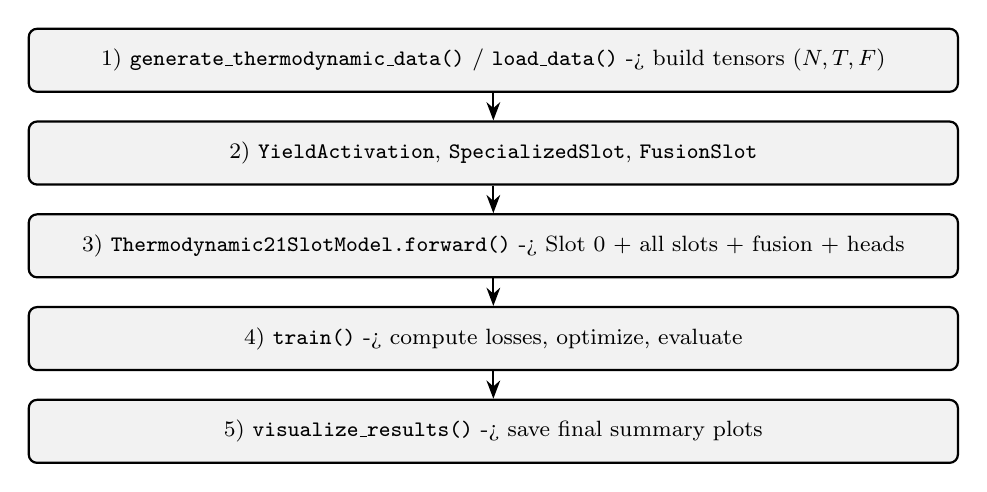
\begin{tikzpicture}[
  node distance=0.7cm,
  cbox/.style={rectangle,rounded corners=3pt,draw,thick,minimum width=11.8cm,minimum height=0.8cm,align=left,font=\footnotesize},
  arr/.style={->,thick,>=Stealth}
]
\node[cbox,fill=gray!10] (a) {1) \texttt{generate\_thermodynamic\_data()} / \texttt{load\_data()}  -> build tensors $(N,T,F)$};
\node[cbox,fill=gray!10,below=0.35cm of a] (b) {2) \texttt{YieldActivation}, \texttt{SpecializedSlot}, \texttt{FusionSlot}};
\node[cbox,fill=gray!10,below=0.35cm of b] (c) {3) \texttt{Thermodynamic21SlotModel.forward()}  -> Slot 0 + all slots + fusion + heads};
\node[cbox,fill=gray!10,below=0.35cm of c] (d) {4) \texttt{train()}  -> compute losses, optimize, evaluate};
\node[cbox,fill=gray!10,below=0.35cm of d] (e) {5) \texttt{visualize\_results()}  -> save final summary plots};

\draw[arr] (a) -- (b);
\draw[arr] (b) -- (c);
\draw[arr] (c) -- (d);
\draw[arr] (d) -- (e);
\end{tikzpicture}
\caption{Execution order of the Python file.}
\end{figure}

% ===========================================================
\section{Code Blocks and Explanation}
% ===========================================================

\subsection{A) Data generation and loading}

\begin{lstlisting}[caption=Data stage]
def load_data():
    if not os.path.exists(os.path.join(DATA_DIR, 'ground_truth.csv')):
        return generate_thermodynamic_data()
    # else: read CSV and reshape to (N, T, F)
\end{lstlisting}

\textbf{Explanation:}
\begin{itemize}
  \item If CSV files do not exist, the script creates physically-informed synthetic data.
  \item Otherwise, it loads data directly and converts to tensors.
  \item This makes the code fully runnable without manual preprocessing.
\end{itemize}

\subsection{B) Physics activation (yield behavior)}

\begin{lstlisting}[caption=YieldActivation]
class YieldActivation(nn.Module):
    def forward(self, x):
        sigma_y = F.softplus(self.sigma_y_raw) + 0.01
        p = 1.5 + F.softplus(self.p_raw)
        ratio = (x / sigma_y).abs().clamp(max=15.0)
        return x / (1.0 + ratio.pow(p)).pow(1.0 / p)
\end{lstlisting}

\[
f(x)=\frac{x}{\left(1+|x/\sigma_y|^p\right)^{1/p}}
\]

\textbf{Explanation:}
\begin{itemize}
  \item For small amplitudes, response is almost linear.
  \item For large amplitudes, response saturates (yield-like behavior).
  \item Each slot learns its own $\sigma_y$ and $p$ from data.
\end{itemize}

\subsection{C) Slot 0: main physics branch}

\begin{lstlisting}[caption=Slot 0 branch]
hm = load[:, :, :2]  # horizontal load H and moment M
slot0_in = torch.cat([hm, pile, soil], dim=-1)
h_slot0 = self.slot0_gmax_hm(slot0_in)
gmax_slot0 = torch.sigmoid(self.slot0_gmax_head(h_slot0).squeeze(-1))
trigger = torch.sigmoid(self.slot0_trigger_head(h_slot0).squeeze(-1))
trigger_state = torch.cummax(trigger, dim=1)[0]
\end{lstlisting}

\textbf{Explanation:}
\begin{itemize}
  \item Slot 0 explicitly combines the most important physical variables.
  \item It predicts an early estimate of $G/G_{\max}$.
  \item It also predicts trigger state $\tau_t$ that is monotonic over time.
\end{itemize}

\subsection{D) Multi-slot fusion and final prediction}

\begin{lstlisting}[caption=Fusion + final G/Gmax]
all_slots = [h_slot0] + load_slots + soil_slots + pile_slots
fused, fusion_attn = self.fusion_slot(all_slots)
x = self.encoder(fused + self.pe[:, :T])

slot_agg = self.slot_gate(torch.cat(all_slots, dim=-1))
x_out = torch.cat([x, slot_agg], dim=-1)

gmax_main = self.head_G_Gmax(x_out).squeeze(-1)
G_Gmax = torch.clamp(0.65 * gmax_main + 0.35 * gmax_slot0, 0.0, 1.0)
\end{lstlisting}

\textbf{Explanation:}
\begin{itemize}
  \item Fusion uses all specialized slots to capture global interactions.
  \item Final $G/G_{\max}$ combines global branch and Slot 0 branch.
  \item This is a balance between expressiveness and physical guidance.
\end{itemize}

\subsection{E) Triggered stiffness drop}

\begin{lstlisting}[caption=Post-processing with trigger]
C_ratio = self.head_C_ratio(x_out).squeeze(-1)
E_diss = self.head_E_diss(x_out).squeeze(-1)

C_ratio = torch.clamp(C_ratio * (1.0 - 0.20 * trigger_state), 0.0, 1.0)
E_diss = torch.clamp(E_diss + 0.10 * trigger_state, 0.0, 1.0)
\end{lstlisting}

\textbf{Explanation:}
\begin{itemize}
  \item When trigger grows, stiffness is reduced more aggressively.
  \item Dissipated energy is increased with trigger.
  \item This encodes irreversible degradation behavior.
\end{itemize}

\subsection{F) Physics-informed loss terms}

\begin{lstlisting}[caption=Main physics losses]
# data terms
L_G = F.mse_loss(G_p, G_t)
L_C = F.mse_loss(C_p, C_t)
L_E = F.mse_loss(E_p, E_t)
L_S = F.mse_loss(S_p, S_t)

# load increase => stiffness decrease
L_mono_C = (F.relu(d_C) * inc_mask).sum() / (inc_mask.sum() + 1e-6)

# thermodynamic consistency
L_E_cons = F.mse_loss(E_p, (1.0 - G_p).clamp(0.0, 1.0))
L_S_cons = F.mse_loss(S_p, -torch.log(G_p.clamp(min=1e-3)))
\end{lstlisting}

\textbf{Compact objective:}
\[
\mathcal{L}=2.2L_G+0.6L_C+0.3L_E+0.2L_S+0.8L_{slot0}+0.8L_{monoC}+0.6L_{trigger}+0.5L_{thermo}
\]

\textbf{Explanation:}
\begin{itemize}
  \item Data losses fit the targets.
  \item Monotonic loss enforces physical direction (load up, stiffness down).
  \item Thermodynamic losses enforce consistency with $E$ and $S$ behavior.
\end{itemize}

\subsection{G) Training and outputs}

\begin{lstlisting}[caption=Training and graph export]
model = Thermodynamic21SlotModel(n_steps=T)
opt = torch.optim.Adam(model.parameters(), lr=LR)

# train loop ...
print_results_legend()
plot_path = visualize_results(model, data, te_idx, losses, comp_hist)
print(f"Saved graphs -> {plot_path}")
\end{lstlisting}

\textbf{Explanation:}
\begin{itemize}
  \item Standard training loop with gradient clipping for stability.
  \item The script prints a terminal legend before showing final summary information.
  \item After evaluation, the script saves one summary plot image.
\end{itemize}

\subsection{H) Runtime legend and improved plot labels}

\begin{lstlisting}[caption=Terminal legend printed at runtime]
def print_results_legend():
    print("RESULTS LEGEND")
    print("G/Gmax    -> Main target (1=stiff, lower=degraded)")
    print("C_ratio   -> Should drop when load increases")
    print("E_diss    -> Should generally increase")
    print("Entropy   -> Should generally increase")
    print("(c) circles=True, squares=Pred")
    print("(f) Heatmap=attention, cyan line=trigger")
\end{lstlisting}

\begin{lstlisting}[caption=Graph legends added in visualization]
# panel (c): explicit legend True vs Pred
ax[0, 2].plot(..., 'o-', label='True')
ax[0, 2].plot(..., 's--', label='Pred')
ax[0, 2].legend(fontsize=8)

# panel (f): colorbar + trigger legend
cbar.set_label('Attention weight')
ax_t.plot(..., color='cyan', label='Trigger')
ax_t.legend(loc='upper right', fontsize=8)
\end{lstlisting}

\textbf{Explanation:}
\begin{itemize}
  \item Results are now self-explained directly when the code runs (terminal legend).
  \item The saved figure is easier to read because true/pred and trigger/attention are explicitly labeled.
\end{itemize}

% ===========================================================
\section{Results Legend and Metric Interpretation}
% ===========================================================

\subsection{Legend for Result Plots}

Use this legend to read the generated result figure (the one saved by the code):
\begin{itemize}
  \item \textbf{(a) Total Training Loss}: global objective over epochs. Lower is better.
  \item \textbf{(b) Loss Components}: separate curves for prediction errors on $G$, $C$, $E$, and $S$.
  \item \textbf{(c) $G/G_{\max}$ vs Time}: circles = ground truth, squares = prediction.
  \item \textbf{(d) $C$ ratio vs Time}: circles = ground truth, squares = prediction.
  \item \textbf{(e) Predicted vs True Scatter}: points closer to the diagonal mean better prediction.
  \item \textbf{(f) Attention/Trigger Panel}: heatmap shows slot importance; brighter color means stronger attention. Trigger line indicates activation intensity over time.
\end{itemize}

\subsection{Meaning of Each Metric}

\renewcommand{\arraystretch}{1.25}
\begin{tabular}{|p{2.0cm}|p{4.6cm}|p{3.4cm}|p{4.0cm}|}
\hline
\textbf{Metric} & \textbf{Definition} & \textbf{Target Trend} & \textbf{Interpretation} \\
\hline
$G/G_{\max}$ & Soil shear modulus ratio (normalized stiffness state) & Decreases with damage/load history & Main output. Near 1 = healthy/stiff soil, lower values = degradation \\
\hline
$C$ ratio & Predicted lateral stiffness ratio & Decreases when load increases & Should follow physical monotonic behavior under stronger loading \\
\hline
$E$ (diss.) & Dissipated energy proxy & Increases with damage & Should be consistent with $E \approx 1-G$ \\
\hline
$S$ (entropy) & Irreversibility proxy & Increases with degradation & Represents thermodynamic irreversibility; should not oscillate downward strongly \\
\hline
MSE & Mean squared error between prediction and target & Lower is better & Primary numerical quality measure for each output \\
\hline
$L_G$ & MSE on $G/G_{\max}$ & Lower is better & Most important supervised term (main task) \\
\hline
$L_C$ & MSE on stiffness ratio $C$ & Lower is better & Measures stiffness prediction accuracy \\
\hline
$L_E$ & MSE on energy output & Lower is better & Measures energy prediction accuracy \\
\hline
$L_S$ & MSE on entropy output & Lower is better & Measures entropy prediction accuracy \\
\hline
$L_{monoC}$ & Penalty when load rises but stiffness also rises & Close to 0 is best & Enforces $\Delta L\uparrow \Rightarrow \Delta C\downarrow$ \\
\hline
$L_{thermo}$ & Thermodynamic consistency term (including $E\approx1-G$ and entropy consistency) & Lower is better & Makes outputs physically coherent, not only numerically fitted \\
\hline
\end{tabular}

\subsection{Quick Reading Rule}

A result is considered physically good when:
\begin{itemize}
  \item training losses decrease and stabilize,
  \item predicted curves follow true curves in panels (c) and (d),
  \item scatter points in panel (e) cluster around the diagonal,
  \item $G$ and $C$ decrease while $E$ and $S$ increase consistently with loading.
\end{itemize}

% ===========================================================
\section{End-to-End Flow (Graphical Summary)}
% ===========================================================

\begin{figure}[htbp]
\centering
\begin{tikzpicture}[
  node distance=0.8cm and 0.7cm,
  step/.style={rectangle,rounded corners=3pt,draw,thick,minimum width=3.0cm,minimum height=0.8cm,align=center,font=\footnotesize},
  arr/.style={->,thick,>=Stealth}
]
\node[step,fill=gray!12] (s1) {Generate/Load data};
\node[step,fill=green!12,right=0.8cm of s1] (s2) {Slot 0 + 19 slots};
\node[step,fill=fusioncolor!12,right=0.8cm of s2] (s3) {Fusion + Encoder};
\node[step,fill=yellow!16,below=0.9cm of s3] (s4) {Predict $G,C,E,S$};
\node[step,fill=blue!12,left=0.8cm of s4] (s5) {Physics losses};
\node[step,fill=gray!12,left=0.8cm of s5] (s6) {Update weights};

\draw[arr] (s1) -- (s2);
\draw[arr] (s2) -- (s3);
\draw[arr] (s3) -- (s4);
\draw[arr] (s4) -- (s5);
\draw[arr] (s5) -- (s6);
\draw[arr] (s6.north) |- (s2.south);
\end{tikzpicture}
\caption{Training cycle of the model.}
\end{figure}

\textbf{Main takeaway:} the code is organized to keep the prediction accurate while forcing physically consistent degradation behavior.

\end{document}
